\chapter{Conditional Distributions and Conditional Expectation}
\makeheading{Week 2}{\daterange{2021-09-15}{2021-09-22}}%chktex 8
\section{Definitions and Construction}
\subsection*{Jointly Discrete Case}
\begin{Regular}
    \textbf{Formulation}: If $ X_1 $ and $ X_2 $ are both discrete rvs with joint pmf $ p(x_1,x_2) $ and
    marginal pmfs $ p_1(x_1) $ and $ p_2(x_2) $, respectively, then the conditional distribution of $ X_1 $
    given $ X_2=x_2 $, denoted by $ X_1\mid (X_2=x_2) $, is defined via its \emph{conditional pmf}
    \[ p_{1\mid 2}(x_1\mid x_2)=\Prob{X_1=x_1\given X_2=x_2}=\frac{\Prob{X_1=x_1,X_2=x_2}}{\Prob{X_2=x_2}}=\frac{p(x_1,x_2)}{p_2(x_2)}, \]
    provided that $ p_2(x_2)>0 $. Similarly, the conditional distribution of $ X_2\mid(X_1=x_1) $ is defined via its conditional pmf
    \[ p_{2\mid 1}(x_2\mid x_1)=\Prob{X_2=x_2\given X_1=x_1}=\frac{p(x_1,x_2)}{p_1(x_1)},\text{ provided that $ p_1(x_1)>0 $.} \]
    \tcblower{}
    \underline{Remarks}:
    \begin{enumerate}[(1)]
        \item If $ X_1 $ and $ X_2 $ are \underline{independent}, then $ p(x_1,x_2)=p_1(x_1)p_2(x_2) $ $ \forall x_1,x_2\in\mathbb{R} $, and so
              $ p_{1\mid 2}(x_1\mid x_2)=p_1(x_1) $ and $ p_{2\mid 1}(x_2\mid x_1)=p_2(x_2) $.
        \item These ideas extend beyond the simple bivariate case naturally. For example,
              suppose that $ X_1 $, $ X_2 $, and $ X_3 $ are discrete rvs. We can define the conditional distribution
              of $ (X_1,X_2) $ given $ X_3=x_3 $ via its conditional pmf as follows:
              \[ p_{12\mid 3}(x_1,x_2\mid x_3)=\frac{\Prob{X_1=x_1,X_2=x_2,X_3=x_3}}{\Prob{X_3=x_3}}=\frac{p(x_1,x_2,x_3)}{p_3(x_3)}, \]
              provided that $ p_3(x_3)>0 $. Alternatively, we can define the conditional distribution of $ X_2 $
              given $ (X_1=x_1,X_3=x_3) $ via its conditional pmf given by
              \[ p_{2\mid 13}(x_2\mid x_1,x_3)=\frac{p(x_1,x_2,x_3)}{p_{13}(x_1,x_3)},\text{ provided that $ p_{13}(x_1,x_3)>0 $,} \]
              where $ p_{13}(x_1,x_3) $ is the joint pmf of $ X_1 $ and $ X_3 $.
    \end{enumerate}
\end{Regular}
\begin{Regular}
    \textbf{Conditional Expectation}: The \emph{conditional mean} of $ X_1\mid(X_2=x_2) $ is
    \[ \E{X_1\given X_2=x_2}=\sum_{x_1}x_1 p_{1\mid 2}(x_1\mid x_2).  \]
    More generally, if $ w(\:\cdot\:,\:\cdot\:) $, $ h(\:\cdot\:) $, and $ g(\:\cdot\:) $ are arbitrary real-valued functions, then
    \[ \E[\big]{w(X_1,X_2)\given X_2=x_2}=\E[\big]{w(X_1,x_2)\given X_2=x_2}=\sum_{x_1}w(x_1,x_2)p_{1\mid 2}(x_1\mid x_2) \]
    and
    \[ \E[\big]{g(X_1)h(X_2)\given X_2=x_2}=\E[\big]{g(X_1)h(x_2)\given X_2=x_2}=h(x_2)\E[\big]{g(X_1)\given X_2=x_2}. \]
    As an immediate consequence, if $ a,b\in\mathbb{R} $, then we obtain
    \[ \E[\big]{ag(X_1)+bh(X_1)\given X_2=x_2}=a\E[\big]{g(X_1)\given X_2=x_2}+b\E[\big]{h(X_1)\given X_2=x_2}. \]
    Furthermore, if we recall that $ \E{X_1+X_2}=\sum_{x_1}\sum_{x_2}(x_1+x_2)p(x_1,x_2) $, then it correspondingly follows that
    \begin{align*}
        \E{X_{1}+X_{2} \given X_{3}=x_{3}}
         & =\sum_{x_{1}} \sum_{x_{2}}(x_{1}+x_{2}) p_{12 \mid 3}(x_{1}, x_{2} \mid x_{3})                                                                                       \\
         & =\sum_{x_{1}} \sum_{x_{2}}(x_{1}+x_{2}) \frac{p(x_{1}, x_{2}, x_{3})}{p_{3}(x_{3})}                                                                                  \\
         & =\sum_{x_{1}} \sum_{x_{2}} x_{1} \cdot \frac{p(x_{1}, x_{2}, x_{3})}{p_{3}(x_{3})}+\sum_{x_{1}} \sum_{x_{2}} x_{2} \cdot \frac{p(x_{1}, x_{2}, x_{3})}{p_{3}(x_{3})} \\
         & =\sum_{x_{1}} \frac{x_{1}}{p_{3}(x_{3})} \sum_{x_{2}} p(x_{1}, x_{2}, x_{3})+\sum_{x_{2}} \frac{x_{2}}{p_{3}(x_{3})} \sum_{x_{1}} p(x_{1}, x_{2}, x_{3})             \\
         & =\sum_{x_{1}} \frac{x_{1}}{p_{3}(x_{3})} p_{13}(x_{1}, x_{3})+\sum_{x_{2}} \frac{x_{2}}{p_{3}(x_{3})} p_{23}(x_{2}, x_{3})                                           \\
         & =\sum_{x_{1}} x_{1} p_{1 \mid 3}(x_{1} \mid x_{3})+\sum_{x_{2}} x_{2} p_{2 \mid 3}(x_{2} \mid x_{3})                                                                 \\
         & =\E{X_1\given X_3=x_3}+\E{X_2\given X_3=x_3}.
    \end{align*}
\end{Regular}
\begin{Regular}
    \textbf{We have}: $ \E{X_1+X_2\given X_3=x_3}=\E{X_1\given X_3=x_3}+\E{X_2\given X_3=x_3} $. In other words, the conditional expected
    value is also a \textbf{linear} operator. In fact, more generally, if $ a_i\in\mathbb{R} $, $ i=1,2,\ldots,n $, then the same essential approach can be used to show that
    \[ \E[\bigg]{\sum_{i=1}^{n} a_i X_i\given Y=y}=\sum_{i=1}^{n} a_i\E{X_i\given Y=y}. \]
\end{Regular}
\begin{Regular}
    \textbf{Conditional Variance}: If we take $ g(X_1)=\bigl(X_1-\E{X_1\given X_2=x_2}\bigr)^2 $, then
    \[ \E[\big]{g(X_1)\given X_2=x_2}=\E[\Big]{\bigl(X_1-\E{X_1\given X_2=x_2}\bigr)^2\given X_2=x_2}=\Var{X_1\given X_2=x_2} \]
    is the \emph{conditional variance} of $ X_1\mid (X_2=x_2) $.
\end{Regular}
As with the calculation of variance, the following result provides an alternative (and often times
preferred) way to calculate $ \Var{X_1\given X_2=x_2} $.
\begin{Result}
    \textbf{Theorem 2.1}. $ \Var{X_1\given X_2=x_2}=\E{X_1^2\given X_2=x_2}-\E{X_1\given X_2=x_2}^2 $.
    \tcblower{}
    \textbf{Proof}:
    \begin{align*}
        \Var{X_1\given X_2=x_2}
         & =\E[\Big]{\bigl(X_1-\E{X_1\given X_2=x_2}\bigr)^2\given X_2=x_2}                 \\
         & =\E[\big]{X_1^2-2X_1\E{X_1\given X_2=x_2}+\E{X_1\given X_2=x_2}^2\given X_2=x_2} \\
         & =\E{X_1^2}-2\E{X_1\given X_2=x_2}^2+\E{X_1\given X_2=x_2}^2                      \\
         & =\E{X_1^2\given X_2=x_2}-\E{X_1\given X_2=x_2}^2
    \end{align*}
\end{Result}
\begin{Example}
    \textbf{Example 2.1}. Suppose that $ X_1 $ and $ X_2 $ are discrete rvs having joint pmf of the form
    \[ p(x_1,x_2)=\begin{cases*}
            1/5  & , if $ x_1=1 $ and $ x_2=0 $, \\
            2/15 & , if $ x_1=0 $ and $ x_2=1 $, \\
            1/15 & , if $ x_1=1 $ and $ x_2=2 $, \\
            1/5  & , if $ x_1=2 $ and $ x_2=0 $, \\
            2/5  & , if $ x_1=1 $ and $ x_2=1 $, \\
            0    & , otherwise.
        \end{cases*} \]
    Find the conditional distribution of $ X_1\mid (X_2=1) $. Also, calculate $ \E{X_1\given X_2=1} $ and
    $ \Var{X_1\given X_2=1} $.
    \tcblower{}
    \textbf{Solution}: Note that for problems of this nature, it often helps to create a table summarizing the information:
    \begin{center}
        \begin{NiceTabular}{cc|ccc|c}
            &\Block{1-5}{$ x_2 $}                                                                                                                        \\%chktex 8
            & $ p(x_1,x_2) $        & $ 0 $                      & $ 1 $                      & $ 2 $                      &$ p_1(x_1) $ \\
            \cmidrule{2-6}
            \Block{3-1}{$ x_1 $}           & $ 0 $                       & $ 0 $                      & $ 2/15 $                   & $ 0 $                      & $ 2/15 $                            \\%chktex 8
            & $ 1 $                       & $ 1/5 $                    & $ 2/5 $                    & $ 1/15 $                   & $ 2/3 $                            \\
            & $ 2 $                       & $ 1/5 $                    & $ 0 $                      & $ 0 $                      & $ 1/5 $                            \\
            \cmidrule{2-6}
            & $ p_2(x_2) $   & $ 2/5 $   & $ 8/15 $ & $ 1/15 $ & $ 1 $
        \end{NiceTabular}
    \end{center}
    Then,
    \begin{itemize}
        \item $ p_{1\mid 2}(0\mid 1)=\Prob{X_1=0\given X_2=1}=(2/15)/(8/15)=1/4 $, and
        \item $ p_{1\mid 2}(1\mid 1)=\Prob{X_1=1\given X_2=1}=(2/5)/(8/15)=3/4 $.
    \end{itemize}
    Thus, the conditional pmf of $ X_1\mid(X_2=1) $ can be
    represented as follows:
    \begin{center}
        \begin{NiceTabular}{c|cc}
            $ x_1 $ & $ 0 $ & $ 1 $\\
            \midrule
            $ p_{1\mid 2}(x_1\mid 1) $ & $ 1/4 $ & $ 3/4 $
        \end{NiceTabular}
    \end{center}
    Note that $ X_1\mid (X_2=1)\sim \BERN{3/4} $. Thus, $ \E{X_1\given X_2=1}=3/4 $ and $ \Var{X_1\given X_2=1}=3/4(1-3/4)=3/16 $.
\end{Example}
\begin{Example}
    \textbf{Example 2.2}. For $ i=1,2 $, suppose that $ X_i \sim \BIN{n_i,p} $ where $ X_1 $ and $ X_2 $ are independent. Find the
    conditional distribution of $ X_1 $ given $ X_1+X_2=m $.
    \tcblower{}
    \textbf{Solution}: We want to find the conditional pmf of $ X_1\mid (Y=m) $, where $ Y=X_1+X_2 $. Let this conditional
    pmf be denoted by $ p_{X_1\mid Y}(x_1\mid m)=\Prob{X_1=x_1\given Y=m} $.
    Recall from Example 1.5 that $ X_1+X_2 \sim \BIN{n_1+n_2,p} $.
    \begin{align*}
        p_{X_1\mid Y}(x_1\mid m)
         & =\frac{\Prob{X_1=x_1,Y=m}}{\Prob{Y=m}}                                                                                               \\
         & =\frac{\Prob{X_1=x_1,X_1+X_2=m}}{\Prob{X_1+X_2=m}}                                                                                   \\
         & =\frac{\Prob{X_1=x_1,X_2=m-x_1}}{\binom{n_1+n_2}{m}p^m (1-p)^{n_1+n_2-m}}                                                            \\
         & =\frac{p_1(x_1)p_2(m-x_1)}{\binom{n_1+n_2}{m}p^m (1-p)^{n_1+n_2-m}}                                                                  \\
         & =\frac{\binom{n_1}{x_1}p^{x_1}(1-p)^{n_1-x_1}\binom{n_2}{m-x_1}p^{m-x_1}(1-p)^{n_2-(m-x_1)}}{\binom{n_1+n_2}{m}p^m(1-p)^{n_1+n_2-m}}
    \end{align*}
    provided that $ 0\le x_1\le n_1 $, and $ 0\le m-x_1\le n_2 $ (i.e., $ m-n_2\le x\le m $). Simplifying,
    \[p_{X_1\mid Y}(x_1\mid m)=\frac{\binom{n_1}{x_1}\binom{n_2}{m-x_1}}{\binom{n_1+n_2}{m}},\]
    for $ x_1=\max{0,m-n_2},\ldots,\min{n_1,m} $.
\end{Example}
\underline{Remark}: Looking at the conditional pmf we just obtained, we recognize that $ X_1\mid(X_1+X_2=m)\sim \HG{n_1+n_2,n_1,m} $.
The result that $ X_1\mid(X_1+X_2=m) $ has a hypergeometric distribution should not be all that surprising. Consider the sequence of $ n_1+n_2 $
Bernoulli trials represented visually as follows:
\[ \underbrace{\begin{matrix}
            \boxed{1} & \boxed{2} & \cdots & \boxed{n_1} & \boxed{1} & \boxed{2} & \cdots & \boxed{n_2}
        \end{matrix}}_{\text{$ n_1+n_2 $ trials}} \]
Of these $ n_1+n_2 $ trials in which $ m $ of them were known to be successes, we want $ x_1 $ successes to have occurred among the first $ n_1 $
trials (thereby implying that $ m-x_1 $ successes are obtained during the final $ n_2 $ trials). Since any of these trials were equally likely to be a success
(i.e., the same success probability $p$ is assumed), the desired result ends up being the obtained
hypergeometric probability.
\begin{Example}
    \textbf{Example 2.3}. Let $ X_1,X_2,\ldots,X_m $ be independent rvs where $ X_i \sim \POI{\lambda_i} $, $ i=1,2,\ldots,m $. Define
    $ Y=\sum_{i=1}^{m} X_i $. Find the conditional distribution of $ X_j\mid(Y=n) $.
    \tcblower{}
    \textbf{Solution}: We are interested in the conditional pmf of $ X_j\mid(Y=n) $, to be denoted by
    \begin{align*}
        p_{X_j\mid Y}(x_j\mid n)
         & =\Prob{X_j=x_j\given Y=n}                                      \\
         & =\frac{\Prob{X_j=x_j, Y=n}}{\Prob{Y=n}}                        \\
         & =\frac{\Prob[\bigg]{X_j=x_j,\sum_{i=1}^{m} X_i=n}}{\Prob{Y=n}}
    \end{align*}
    First, we investigate the numerator:
    \begin{align*}
        \Prob[\bigg]{X_j=x_j,\sum_{i=1}^{m} X_i=n}
         & =\Prob[\bigg]{X_j=x_j,X_j+\sum_{i=1,i\ne j}^m X_i=n}         \\
         & =\Prob[\bigg]{X_j=x_j,\sum_{i=1,i\ne j}^m X_i=n-x_j}         \\
         & =\Prob{X_j=x_j}\Prob[\bigg]{\sum_{i=1,i\ne j}^{m} X_i=n-x_j}
    \end{align*}
    where the last equality follows due to the independence of $ \Set{X_i}_{i=1}^m $. We are given that
    $ X_j \sim \POI{\lambda_j} $. Due to the result of Exercise 1.1, it follows that
    \[ \sum_{i=1,i\ne j}^{m} X_i \sim \POI[\bigg]{\sum_{i=1,i\ne j}^{m} \lambda_i}. \]
    By the same result, we also have that
    \[ Y=\sum_{i=1}^{m} X_i \sim \POI[\bigg]{\sum_{i=1}^{m} \lambda_i}. \]
    Therefore,
    \begin{align*}
        p_{X_j\mid Y}(x_j\mid n)
         & =\frac{\frac{e^{-\lambda_j}\lambda_j^{x_j}}{x_j!}\frac{e^{-\sum_{i=1,i\ne j}^{m} \lambda_i}(\sum_{i=1,i\ne j}^{m}\lambda_i)^{n-x_j}}{(n-x_j)}}{\frac{e^{-\sum_{i=1}^{m} \lambda_i}(\sum_{i=1}^{m} \lambda_i)^n}{n!}}
    \end{align*}
    provided that $ x_j\ge 0 $ and $ n-x_j\ge 0 $ which implies $ 0\le x_j\le n $. Thus,
    \begin{align*}
        p_{X_j\mid Y}(x_j\mid n)
         & =\binom{n}{x_j}\frac{\lambda_j^{x_j}(\lambda_Y-\lambda_j)^{n-x_j}}{\lambda_Y^n}                                                       \\
         & =\binom{n}{x_j}\biggl(\frac{\lambda_j}{\lambda_Y}\biggr)^{x_j}\biggl(1-\frac{\lambda_j}{\lambda_Y} \biggr)^{n-x_j},\;x_j=0,1,\ldots,n
    \end{align*}
    where $ \lambda_Y=\sum_{i=1}^{m} \lambda_i $ and note that $ \lambda_Y^{x_j}\lambda_Y^{n-x_j}=\lambda_Y $. We see that
    \[ X_j\mid (Y=n)\sim \BIN[\bigg]{n,\frac{\lambda_j}{\sum_{i=1}^{m} \lambda_i}}. \]
\end{Example}
\begin{Example}
    \textbf{Example 2.4}. Suppose that $ X \sim \POI{\lambda} $ and $ Y\mid(X=x)\sim \BIN{x,p} $. Find the conditional distribution of $ X\mid(Y=y) $.
    \tcblower{}
    \textbf{Solution}: We want to calculate the conditional pmf of $ X\mid(Y=y) $, to be denoted by
    \[ p_{X\mid Y}(x\mid y)=\Prob{X=x\given Y=y}=\frac{\Prob{X=x,Y=y}}{\Prob{Y=y}}. \]
    First, note that
    \[ \Prob{Y=y\given X=x}=\frac{\Prob{X=x,Y=y}}{\Prob{X=x}}, \]
    which implies that
    \[ \Prob{X=x,Y=y}=\Prob{Y=y\given X=x}\Prob{X=x}=\frac{e^{-\lambda}\lambda^x}{x!}\binom{x}{y}p^y(1-p)^{x-y},  \]\
    for $x=0,1,2,\ldots$ and $y=0,1,\ldots,x$.
    Note that the range of $ y $ depends on the values of $ x $. A graphical display of the region is given below:
    \begin{center}
        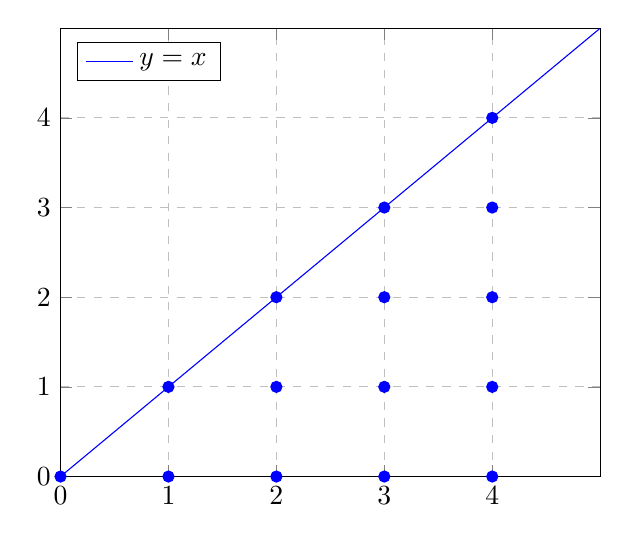
\begin{tikzpicture}
            \begin{axis}[
                    xmin=0, xmax=5,
                    ymin=0, ymax=5,
                    xtick={0,1,2,3,4},
                    ytick={0,1,2,3,4},
                    legend pos=north west,
                    ymajorgrids=true,
                    xmajorgrids=true,
                    grid style=dashed,
                ]
                \addplot[color=blue]{x};
                \addplot[color=blue,mark=*,only marks]
                coordinates {
                        (1,0)(2,0)(3,0)(4,0)(2,1)(3,1)(3,2)(4,1)(4,2)(4,3)(0,0)(1,1)(2,2)(3,3)(4,4)
                    };
                \legend{$y=x$}
            \end{axis}
        \end{tikzpicture}
    \end{center}
    We may rewrite this region with the range of $ x $ depending on the values of $ y $. Specifically, note that $ x=0,1,2,\ldots $ and $ y=0,1,\ldots,x $
    is equivalent to $ y=0,1,2,\ldots $ and $ x=y,y+1,y+2,\ldots $. We use this alternative region to find the marginal pmf of $ Y $.
    \begin{align*}
        \Prob{Y=y}
         & =\sum_x\Prob{X=x,Y=y}                                                                                                                \\
         & =\sum_{x=y}^{\infty} e^{-\lambda}\frac{\lambda^x}{x!} \binom{x}{y}p^y(1-p)^{x-y}                                                     \\
         & =\sum_{x=y}^{\infty} e^{-\lambda}\frac{\lambda^x}{x!} \frac{x!}{y!(x-y)!} p^y(1-p)^{x-y}                                             \\
         & =\frac{e^{-\lambda}}{y!} p^y \sum_{x=y}^\infty \frac{\lambda^x (1-p)^{x-y}}{(x-y)!}\lambda^{-y}\lambda^{y}                           \\
         & =\frac{e^{-\lambda}(\lambda p)^y}{y!}\sum_{x=y}^\infty \frac{\bigl(\lambda(1-p)\bigr)^{x-y}}{(x-y)!}       &  & \text{let $ z=x-y $} \\
         & =\frac{e^{-\lambda}(\lambda p)^y}{y!}e^{\lambda(1-p)}                                                                                \\
         & =\frac{e^{-\lambda p}(\lambda p)^y}{y!}                                                                    &  & y=0,1,2,\ldots
    \end{align*}
    In fact, $ Y \sim \POI{\lambda p} $. Therefore,
    \begin{align*}
        p_{X\mid Y}(x\mid y)
         & =\frac{ \frac{e^{-\lambda}\lambda^x}{x!} \frac{x!}{y!(x-y)!} p^y(1-p)^{x-y} }{\frac{e^{-\lambda p}(\lambda p)^y}{y!}} \\
         & =\frac{e^{-\lambda(1-p)}\bigl(\lambda(1-p)\bigr)^{x-y}}{(x-y)!},
    \end{align*}
    for $ x=y,y+1,\ldots $.
\end{Example}
\underline{Remark}: The above conditional pmf is recognized as that of a \textbf{shifted} Poisson distribution ($ y $ units to the right).
Specifically, we have that
\[ X\mid(Y=y)\sim W+y \]
where $ W \sim \POI[\big]{\lambda(1-p)} $.
\begin{Regular}
    \textbf{Formulation}: In the jointly discrete case, it was natural to define:
    \[ p_{X\mid Y}(x\mid y)=\Prob{X=x\given Y=y}=\Prob{X=x,Y=y}/\Prob{Y=y}. \]
    Strictly speaking, this no longer makes sense in a continuous context since $ f(x,y)\ne \Prob{X=x,Y=y} $ and
    $ f_Y(y)\ne \Prob{Y=y} $. However, for small positive values of $ \odif{y} $ (as the figure below shows),
    $ \Prob{y\le Y\le y+\odif{y}}\approx f_Y(y)\odif{y} $.
\end{Regular}
Formally,
\[ f_Y(y)=\lim\limits_{{\odif{y}} \to {0}}\frac{\Prob{y\le Y\le y+\odif{y}}}{\odif{y}}. \]
Similarly,
\[ f(x,y)=\lim\limits_{\odif{x}\to 0,\odif{y}\to 0}\frac{\Prob{x\le X\le x+\odif{x},y\le Y\le y+\odif{y}}}{\odif{x,y}},   \]
which implies that $ \Prob{x\le X\le x+\odif{x},y\le Y\le y+\odif{y}}\approx f(x,y)\odif{x,y} $. For small positive values of
$ \odif{x} $ and $ \odif{y} $, consider now
\begin{align*}
    \Prob{x\le X\le x+\odif{x}\given y\le Y\le y+\odif{y}}
     & =\frac{\Prob{x\le X\le x+\odif{x}\given y\le Y\le y+\odif{y}}}{\Prob{y\le Y\le y+\odif{y}}} \\
     & \approx \frac{f(x,y)\odif{x,y}}{f_Y(y)\odif{y}}                                             \\
     & =\frac{f(x,y)}{f_Y(y)} \odif{x}.
\end{align*}
As a result, we formally define the \emph{conditional pdf} of $ X $ given $ Y=y $ (again to be denoted by $ X\mid(Y=y) $) as
\[ f_{X\mid Y}(x\mid y)=\frac{f(x,y)}{f_Y(y)}=\lim\limits_{\odif{x}\to 0,\odif{y}\to 0}\frac{\Prob{x\le X\le x+\odif{x},y\le Y\le y+\odif{y}}}{\odif{x}}.  \]
\underline{Remark}: In the jointly continuous case, the conditional probability of an event of the form $ \Set{a\le X\le b} $ given $ Y=y $
would be calculated as
\[ \Prob{a\le X\le b\given Y=y}=\int_{a}^{b}f_{X\mid Y}(x\mid y)\odif{x}=\frac{\int_{a}^{b}f(x,y)\odif{x}}{f_Y(y)}, \]
which we can also express as
\[ \Prob{a\le X\le b\mid Y=y}=\frac{\int_{a}^{b}f(x,y)\odif{x}}{\int_{-\infty}^{\infty}f(x,y)\odif{x}}.  \]
In other words, we could view this as a way of assigning probability to an event
$ \Set{a\le X\le b} $ over a ``slice,'' $ Y=y $, of the (joint) region of support for the pair of rvs $ X $ and $ Y $.
\begin{Example}
    \textbf{Example 2.5}. Suppose that the joint pdf of $ X $ and $ Y $ is given by
    \[ f(x,y)=\begin{cases*}
            5e^{-3x-y}, & \text{if $ 0\le 2x\le y< \infty $,} \\
            0,          & \text{elsewhere}.
        \end{cases*} \]
    Determine the conditional distribution of $ Y\mid(X=x) $ where $ 0\le x< \infty $.
    \tcblower{}
    \textbf{Solution}: We wish to find the conditional pdf of $ Y\mid(X=x) $ given by
    \[f_{Y\mid X}(y\mid x)=\frac{f(x,y)}{f_X(x)}\]
    The region of support for this joint distribution looks like:
    \begin{center}
        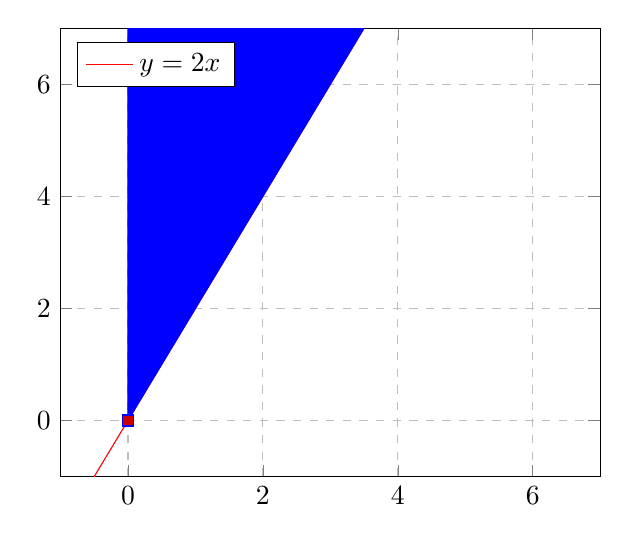
\begin{tikzpicture}
            \begin{axis}[
                    xmin=-1, xmax=7,
                    ymin=-1, ymax=7,
                    legend pos=north west,
                    ymajorgrids=true,
                    xmajorgrids=true,
                    grid style=dashed,
                ]
                \addplot[color=red]{2*x};
                \addplot+ [fill,color=blue] coordinates {
                        (0,0) (6,12) (0,12) (0,0)
                    }
                --cycle
                ;
                \legend{$y=2x$}
            \end{axis}
        \end{tikzpicture}
    \end{center}
    For $ 0<x<\infty $:
    \begin{align*}
        f_X(x)
         & =\int_{-\infty}^{\infty}f(x,y)\odif{y}             \\
         & =\int_{2x}^{\infty}5e^{-3x-y}\odif{y}              \\
         & =\biggl[5e^{-3x}(-e^{-y})\biggr]_{y=2x}^{y=\infty} \\
         & =5e^{-3x}e^{-2x}                                   \\
         & =5e^{-5x}
    \end{align*}
    Note that $ X \sim \EXP{5} $. Finally, we get:
    \[ f_{Y\mid X}(y\mid x)=\frac{5e^{-3x-y}}{5e^{-5x}}=e^{-y+2x},\; y> 2x.  \]
\end{Example}
\underline{Remark}: The conditional pdf of $ Y\mid (X=x) $ is recognized as that of a \emph{shifted exponential distribution}
($2x$ units to the right). Specifically, we have that $ Y\mid(X=x) \sim W+2x $, where $ W \sim \EXP{1} $.
\begin{Regular}
    \textbf{Conditional Expectation}: If $ X $ and $ Y $ are jointly continuous rvs and $ g(\:\cdot\:) $ is an arbitrary
    real-valued function, then the \emph{conditional expectation} of $ g(X) $ given $ Y=y $ is
    \[ \E{g(X)\given Y=y}=\int_{-\infty}^{\infty}g(x)f_{X\mid Y}(x\mid y)\odif{x}, \]
    and so the conditional mean of $ X\mid(Y=y) $ is given by
    \[ \E{X\given Y=y}=\int_{-\infty}^{\infty}x f_{X\mid Y}(x\mid y)\odif{x}. \]
\end{Regular}
\begin{Example}
    \textbf{Example 2.6}. Suppose that the joint pdf of $ X $ and $ Y $ is given by
    \[ f(x,y)=\begin{dcases}
            \frac{12}{5}x(2-x-y), & \text{if $ 0<x<1 $ and $ 0<y<1 $,} \\
            0,                    & \text{elsewhere}.
        \end{dcases} \]
    Find the conditional distribution of $ X $ given $ Y=y $ where $ 0<y<1 $, and use it to calculate its conditional mean.
    \tcblower{}
    \textbf{Solution}: Using our earlier theory, we wish to find the conditional pdf of $ X\mid(Y=y) $ given by
    \[ f_{X\mid Y}(x\mid y)=\frac{f(x,y)}{f_Y(y)}. \]
    The region of support for this joint distribution of $ X $ and $ Y $ look like:
    \begin{center}
        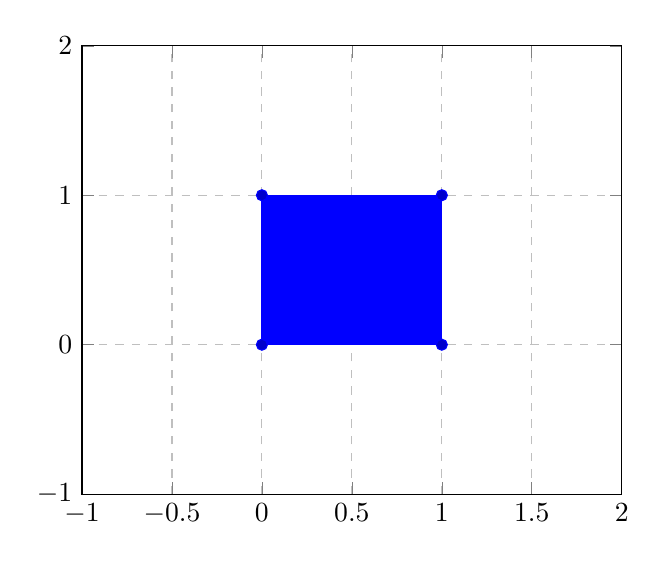
\begin{tikzpicture}
            \begin{axis}[
                    xmin=-1, xmax=2,
                    ymin=-1, ymax=2,
                    legend pos=north west,
                    ymajorgrids=true,
                    xmajorgrids=true,
                    grid style=dashed,
                ]
                \addplot+ [fill] coordinates {
                        (0,0) (0,1) (1,1) (1,0)
                    }
                --cycle
                ;
            \end{axis}
        \end{tikzpicture}
    \end{center}
    For $ 0<y<1 $,
    \begin{align*}
        f_Y(y)
         & =\int_{-\infty}^{\infty}f(x,y)\odif{x}                                     \\
         & =\int_{0}^{1}\frac{12}{5} x(2-x-y)\odif{x}                                 \\
         & =\frac{12}{5} \int_{0}^{1}(2x-x^2-xy)\odif{x}                              \\
         & =\frac{12}{5} \biggl[x^2-\frac{x^3}{3} -\frac{x^2y}{3} \biggr]_{x=0}^{x=1} \\
         & =\frac{12}{5} \biggl(1-\frac{1}{3} -\frac{y}{2} \biggr)                    \\
         & =\frac{2(4-3y)}{5}
    \end{align*}
    You can verify this by integrating $ f_Y(y) $ over the support of $ Y $ (to get $1$). Thus,
    \[ f_{X\mid Y}(x\mid y)=\frac{12/5 x(2-x-y)}{2/5 (4-3y)}=\frac{6x(2-x-y)}{4-3y},\; 0<x<1 \]
    The conditional mean of $ X $ given $ Y=y $ is:
    \begin{align*}
        \E{X\given Y=y}
         & =\int_{0}^{1}x \frac{6x(2-x-y)}{4-3y} \odif{x}                                           \\
         & =\frac{6}{4-3y} \int_{0}^{1}(2x^2-x^3-x^2y)\odif{x}                                      \\
         & =\frac{6}{4-3y} \biggl[\frac{2x^3}{3} -\frac{x^4}{4} -\frac{x^3 y}{3}\biggr]_{x=0}^{x=1} \\
         & =\frac{6}{4-3y} \biggl(\frac{2}{3}-\frac{1}{4}-\frac{y}{3} \biggr)                       \\
         & =\frac{5-4y}{2(4-3y)}
    \end{align*}
\end{Example}
\begin{Regular}
    \textbf{Conditional Variance}: Likewise, as in the jointly discrete case, we can also consider the notion of
    conditional variance, which retains the same definition as before:
    \[ \Var{X\mid Y=y}=\E*{\bigl(X-\E{X\given Y=y}\bigr)^2\given Y=y}=\E{X^2\given Y=y}-\E{X\given Y=y}^2. \]
    A fact that is becoming more and more evident is that conditional expectation inherits many
    of the properties from regular expectation. Moreover, the same properties concerning
    conditional expectation that held in the jointly discrete case continue to hold true in the
    jointly continuous case (as we are effectively replacing summation with integration).
\end{Regular}
\begin{Example}
    \textbf{Example 2.6}. (\emph{continued}) Calculate $ \Var{X\given Y=y} $ where $ 0<y<1 $ and the joint pdf of
    $ X $ and $ Y $ is given by
    \[ f(x,y)=\begin{dcases}
            \frac{12}{5}x(2-x-5), & \text{if $ 0<x<1 $ and $ 0<y<1 $,} \\
            0,                    & \text{elsewhere}.
        \end{dcases} \]
    \tcblower{}
    \textbf{Solution}: Our earlier results tell us that
    \begin{align*}
        \E{X^2\given Y=y}
         & =\int_{0}^{1}x^2 \frac{6x(2-x-y)}{4-3y} \odif{x}                                         \\
         & =\frac{6}{4-3y} \int_{0}^{1}(2x^3-x^4-x^3y)\odif{x}                                      \\
         & =\frac{6}{4-3y} \biggl[\frac{x^4}{2} -\frac{x^5}{5} -\frac{x^4 y}{4} \biggr]_{x=0}^{x=1} \\
         & =\frac{6}{4-3y} \biggl(\frac{1}{2} -\frac{1}{5} -\frac{y}{4} \biggr)                     \\
         & =\frac{3(6-5y)}{10(4-3y)}.
    \end{align*}
    Therefore, this leads to
    \begin{align*}
        \Var{X\given Y=y}
         & =\E{X^2\given Y=y}-\E{X\given Y=y}^2                  \\
         & =\frac{3(6-5y)}{10(4-3y)} -\frac{(5-4y)^2}{4(4-3y)^2} \\
         & =\frac{19+2y(5y-14)}{20(4-3y)^2}.
    \end{align*}
\end{Example}
\subsection*{Mixed Case}
\begin{Regular}
    We can also consider conditional distributions where the rvs are neither jointly continuous nor
    jointly discrete. To consider such a situation, suppose $X$ is a continuous rv having pdf $ f_X(x) $
    and $Y$ is a discrete rv having pmf $ p_Y(y) $.

    If we focus on the conditional distribution of $ X $ given $ Y=y $, then let us look at the following quantity:
    \begin{align*}
        \frac{\Prob{x\le X\le x+\odif{x}\given Y=y}}{\odif{x}}
         & =\frac{\Prob{x\le X\le x+\odif{x},Y=y}}{\odif{x}\Prob{Y=y}}                                            \\
         & = \frac{\Prob{x\le X\le x+\odif{x}}\Prob{Y=y\given x\le X\le x+\odif{x}}}{\odif{x}\Prob{Y=y}}          \\
         & =\frac{\Prob{Y=y\given x\le X\le x+\odif{x}}}{\Prob{Y=y}}\frac{\Prob{x\le X\le x+\odif{x}}}{\odif{x}},
    \end{align*}
    where $ \odif{x} $ is again, a small positive value.

    By letting $ \odif{x}\to 0 $, we can formally define the conditional pdf of $ X\mid(Y=y) $ as follows:
    \begin{align*}
        f(x\mid y)
         & =\lim\limits_{{\odif{x}} \to {0}} \frac{\Prob{x\le X\le x+\odif{x}\given Y=y}}{\odif{x}}                                               \\
         & = \lim\limits_{{\odif{x}} \to {0}}\frac{\Prob{Y=y\given x\le X\le x+\odif{x}}}{\Prob{Y=y}}\frac{\Prob{x\le X\le x+\odif{x}}}{\odif{x}} \\
         & =\frac{\Prob{Y=y\given X=x}}{\Prob{Y=y}} f_X(x)                                                                                        \\
         & =\frac{p(y\mid x)f_X(x)}{p_Y(y)},
    \end{align*}
    where $ p(y\mid x)=\Prob{Y=y\given X=x} $ is defined as the conditional pmf of $ Y\mid(X=x) $. Note that
    since $ f(x\mid y) $ is a pdf, it follows that
    \[ \int_{-\infty}^{\infty}f(x\mid y)\odif{x} =1\implies p_Y(y)=\int_{-\infty}^{\infty}p(y\mid x)f_X(x)\odif{x}. \]
    Similarly, we can also write
    \[ p(y\mid x)=\frac{f(x\mid y)p_Y(y)}{f_X(x)}. \]
    Since $ p(y\mid x) $ is a pmf, we have that
    \[ \sum_y p(y\mid x)=1\implies f_X(x)=\sum_y f(x\mid y)p_Y(y). \]
\end{Regular}
\begin{Example}
    \textbf{Example 2.7}. Suppose that $ X \sim \U{0,1} $ and $ Y\mid(X=x)\sim \BERN{x} $. Find the conditional distribution of $ X\mid(Y=y) $.
    \tcblower{}
    \textbf{Solution}: We wish to find the conditional pdf of $ X\mid (Y=y) $ given by
    \[ f(x\mid y)=\frac{p(y\mid x)f_X(x)}{p_Y(y)} \]
    Based on the given information, we have
    \begin{align*}
        f_X(x)     & =1,\;0<x<1,              \\
        p(y\mid x) & =x^y(1-x)^{1-y},\;y=0,1.
    \end{align*}
    For $ y=0,1 $, note that
    \begin{align*}
        p_Y(y)
         & =\int_{-\infty}^{\infty}p(y\mid x)f_X(x)\odif{x} \\
         & =\int_{0}^{1}x^y (1-x)^{1-y}(1)\odif{x}
    \end{align*}
    \begin{itemize}
        \item For $ y=0\implies p_Y(0)=\int_{0}^{1}(1-x)\odif{x}=\bigl[x-x^2/2\bigr]_{x=0}^{x=1}=1/2 $.
        \item For $ y=1\implies p_Y(1)=\int_{0}^{1}x\odif{x}=\bigl[x^2/2\bigr]_{x=0}^{x=1}=1/2 $.
    \end{itemize}
    In other words, we have that
    \[ p_Y(y)=\frac{1}{2} ,\; y=0,1\implies Y \sim \BERN*{\frac{1}{2} } \]
    Thus, for $ y=0,1 $, we ultimately obtain
    \[ f(x\mid y)=\frac{x^y(1-x)^{1-y}(1)}{1/2}=2x^y(1-x)^{1-y},\; 0<x<1. \]
\end{Example}
\section{Computing Expectation by Conditioning}
\subsection*{An Important Observation}
As before, let $ g(\:\cdot\:) $ be an arbitrary real-valued function. In general, we recognize that $ \E[\big]{g(X)\given Y=y}=v(y) $,
where $ v(y) $ is some function of $ y $. With this in mind, let us make the following definition:
\[ \E[\big]{g(X)\given Y}=\E[\big]{g(X)\given Y=y}\big\rvert_{y=Y}=v(Y). \]
Functions of rvs are, once again, rvs themselves. Therefore, it makes sense to consider the
expected value of $v(Y)$. In this regard, we would obtain:
\begin{align*}
    \E*{\E[\big]{g(X)\given Y}}
     & =\E[\big]{v(Y)}                                                                            \\
     & =\begin{cases*}
            \sum_y v(y)p_Y(y)                         & , if $ Y $ is discrete,   \\
            \int_{-\infty}^{\infty}v(y)f_Y(y)\odif{y} & , if $ Y $ is continuous,
        \end{cases*}                     \\
     & =\begin{cases*}
            \sum_y\E[\big]{g(X)\given Y=y}p_Y(y)                          & , if $ Y $ is discrete,   \\
            \int_{-\infty}^{\infty}\E[\big]{g(X)\given Y=y}f_Y(y)\odif{y} & , if $ Y $ is continuous.
        \end{cases*}
\end{align*}
\subsection*{Law of Total Expectation}
The following important result is regarded as the \emph{law of total expectation}.
\begin{Result}
    \textbf{Theorem 2.2}. For rvs $ X $ and $ Y $, $ \E[\big]{g(X)}=\E*{\E[\big]{g(X)\given Y}} $.
    \tcblower{}
    \textbf{Proof}: Without loss of generality, assume that $ X $ and $ Y $ are jointly continuous
    rvs. From above, we have
    \begin{align*}
        \E*{\E[\big]{g(X)\given Y}}
         & =\int_{-\infty}^{\infty}\E[\big]{g(X)\given Y=y}f_Y(y)\odif{y}                                 \\
         & =\int_{-\infty}^{\infty}\int_{-\infty}^{\infty}g(x)f_{X\mid Y}(x\mid y)\odif{x} f_Y(y)\odif{y} \\
         & =\int_{-\infty}^{\infty}\int_{-\infty}^{\infty}g(x)\frac{f(x,y)}{f_Y(y)} f_Y(y)\odif{x,y}      \\
         & =\int_{-\infty}^{\infty}\int_{-\infty}^{\infty}g(x)f(x,y)\odif{y,x}                            \\
         & =\int_{-\infty}^{\infty}g(x)\int_{-\infty}^{\infty}f(x,y)\odif{y} \odif{x}                     \\
         & =\int_{-\infty}^{\infty}g(x)f_X(x)\odif{x}                                                     \\
         & =\E[\big]{g(X)}
    \end{align*}
\end{Result}
\underline{Remark}: Using a similar method of proof, the result of Theorem 2.2 can naturally be extended
as follows:
\[ \E[\big]{g(X,Y)}=\E*{\E[\big]{g(X,Y)\given Y}}. \]
The usefulness of the law of total expectation is well-demonstrated in the following example.
\begin{Example}
    \textbf{Example 2.8}. Suppose that $ X \sim \GEOt{p} $ with pmf $ p_X(x)=(1-p)^{x-1}p $, $ x=1,2,3,\ldots $.
    Calculate $ \E{X} $ and $ \Var{X} $ using the law of total expectation.
    \tcblower{}
    \textbf{Solution}: With $ X \sim \GEOt{p} $, recall that $ X $ actually models the number of (independent) trials
    necessary to obtain the first success. Define:
    \[ Y=\begin{cases*}
            0 & , if the $1\textsuperscript{st}$ trial is a failure, \\
            1 & , if the $1\textsuperscript{st}$ trial is a success.
        \end{cases*} \]
    We observe that $ Y \sim \BERN{p} $, so that $ p_Y(0)=1-p $ and $ p_Y(1)=p $.

    \underline{Note}:
    \begin{itemize}
        \item $ X\mid(Y=1) $ is degenerate at $ 1 $ (i.e., $ X $ given $ Y=1 $ is equal to $ 1 $ with probability $ 1 $).
        \item $ X\mid(Y=0) $ is equivalent in distribution $ 1+X $ (i.e., $ X\mid(Y=0)\sim 1+X $).
    \end{itemize}
    By the law of total expectation, we obtain:
    \begin{align*}
        \E{X}
         & =\E[\big]{\E{X\given Y}}               \\
         & =\sum_{y=0}^{1} \E{X\given Y=y}p_Y(y)  \\
         & =(1-p)\E{X\given Y=y}p_Y(y)            \\
         & =(1-p)\E{X\given Y=0}+p\E{X\given Y=1} \\
         & =(1-p)\E{1+X}+p                        \\
         & =(1-p)+(1-p)\E{X}+p                    \\
         & =1+(1-p)\E{X},
    \end{align*}
    which implies that $ (1-(1-p))\E{X}=1 $, or simply $ \E{X}=1/p $. Similarly, we use the law of total expectation
    to get
    \begin{align*}
        \E{X^2}
         & =\E[\big]{\E{X^2\given Y}}                 \\
         & =\sum_{y=0}^{1} \E{X^2\given Y=y}p_Y(y)    \\
         & =(1-p)\E{X^2\given Y=0}+p\E{X^2\given Y=1} \\
         & =(1-p)\E[\big]{(1+X)^2}+p                  \\
         & =(1-p)\bigl(\E{X^2}+2\E{X}+1\bigr)+p       \\
         & =1+(1-p)\E{X^2}+\frac{2(1-p)}{p},
    \end{align*}
    which implies that
    \[ \bigl(1-(1-p)\bigr)\E{X}=\frac{p+2(1-p)}{p} \]
    or simply
    \[ \E{X^2}=\frac{p+2-2p}{p^2}=\frac{2-p}{p^2} \]
    Finally,
    \[ \Var{X}
        =\frac{2-p}{p^2} -\biggl(\frac{1}{p} \biggr)^2
        =\frac{1-p}{p^2}\]
\end{Example}
\underline{Remarks}:
\begin{enumerate}[(1)]
    \item Note that the obtained mean and variance agree with known results. Moreover, the above
          procedure relied only on basic manipulations and did not involve any complicated sums or
          the differentiation of a mgf.
    \item As part of the above solution, we claimed that $ X\mid(Y=0)\sim Z $ where $ Z=1+X $,
          and this implied that $ \E{X^2\given Y=0}=\E[\big]{(1+X)^2} $. To see why this holds true formally,
          consider first
          \[ p_{X\mid Y}(x\mid 0)=\Prob{X=x\given Y=0}=\frac{\Prob{X=x,Y=0}}{\Prob{Y=0}}=\frac{\Prob{X=x,Y=0}}{1-p}.   \]
          Note that
          \begin{align*}
              \Prob{X=x,Y=0}
               & =\Prob{\text{$1\textsuperscript{st}$ trial is a failure and $ x $ total trials needed to get $1\textsuperscript{st}$ success}}              \\
               & =\Prob{\text{$1\textsuperscript{st}$ trial is a failure, next $ x-2 $ trials are failures, and $x\textsuperscript{th}$ trial is a success}} \\
               & =(1-p)(1-p)^{x-2}p\text{ due to independence of trials.}
          \end{align*}
          Thus,
          \[ p_{X\mid Y}(x\mid 0)=\frac{(1-p)(1-p)^{x-2}p}{1-p}=(1-p)^{x-2}p,\;x=2,3,4,\ldots.  \]
          On the other hand, note that
          \begin{align*}
              p_Z(z)
               & =\Prob{Z=z}                     \\
               & =\Prob{1+X=z}                   \\
               & =\Prob{X=z-1}                   \\
               & =(1-p)^{(z-1)-1}p               \\
               & =(1-p)^{z-2}p,\;z=2,3,4,\ldots.
          \end{align*}
          Since these two pmfs are identical, it follows that $ X\mid(Y=0)\sim Z $. As a further consequence,
          for an arbitrary real-valued function $ g(\:\cdot\:) $, we must have that
          \[ \E[\big]{g(X)\given Y=0}=\E[\big]{g(Z)}=\E[\big]{g(1+X)}. \]
\end{enumerate}
\subsection*{Computing Variances by Conditioning}
\begin{Regular}
    In recognizing that $ \E[\big]{g(X)\given Y=y} $ is a function of $ y $, it similarly
    follows that $ \Var{X\given Y=y} $ is also a function of $ y $. Therefore, we can make the
    following definition:
    \[ \Var{X\given Y}=\Var{X\given Y=y}\bigr\rvert_{y=Y}. \]
    Since $ \Var{X\given Y} $ is a function of $ Y $, it is a rv as well, meaning that we could take its expected
    value. The following result, usually referred to as the \emph{conditional variance formula}, provides a
    convenient way to calculate variance through the use of conditioning.
\end{Regular}
\begin{Result}
    \textbf{Theorem 2.3}. For rvs $ X $ and $ Y $, $ \Var{X}=\E[\big]{\Var{X\given Y}}+\Var[\big]{\E{X\given Y}} $.
    \tcblower{}
    \textbf{Proof}: First, consider the term $ \E[\big]{\Var{X\given Y}} $. Since
    \[ \Var{X\given Y=y}=\E{X^2\given Y=y}-\E{X\given Y=y}^2, \]
    it follows that
    \[ \Var{X\given Y}=\E{X^2\given Y}-\E{X\given Y}^2, \]
    which yields (by Theorem 2.2)
    \begin{align*}
        \E[\big]{\Var{X\given Y}}
         & =\E[\big]{\E{X^2\given Y}-\E{X\given Y}^2}           \\
         & =\E[\big]{\E{X^2\given Y}}-\E[\big]{\E{X\given Y}^2} \\
         & =\E{X^2}-\E[\big]{\E{X\given Y}^2}.
    \end{align*}
    Next, recall
    \[ \Var{v(Y)}=\E[\big]{v(Y)^2}-\E[\big]{v(Y)}^2. \]
    Applying Theorem 2.2 once more,
    \begin{align*}
        \Var[\big]{\E{X\given Y}}
         & =\E[\big]{\E{X\given Y}^2}-\E[\big]{\E{X\given Y}}^2 \\
         & =\E[\big]{\E{X\given Y}^2}-\E{X}^2.
    \end{align*}
    Thus,
    \begin{align*}
        \E[\big]{\Var{X\given Y}}+\Var[\big]{\E{X\given Y}}
         & =\E{X^2}-\E[\big]{\E{X\given Y}^2}+\E[\big]{\E{X\given Y}^2}-\E{X}^2 \\
         & =\E{X^2}-\E{X}^2                                                     \\
         & =\Var{X}.
    \end{align*}
\end{Result}
\begin{Example}
    \textbf{Example 2.9}. Suppose that $ \Set{X_i}_{i=1}^\infty $ is an iid sequence of rvs with common mean $ \mu $
    and common variance $ \sigma^2 $. Let $ N $ be a discrete, non-negative integer-valued rv that
    is independent of each $ X_i $. Find the mean and variance of $ T=\sum_{i=1}^{N} X_i $
    (referred to as a \emph{random sum}).
    \tcblower{}
    \textbf{Solution}: By the law of total expectation,
    \[ \E{T}=\E[\big]{\E{T\given N}}. \]
    Note that
    \begin{align*}
        \E{T\given N=n}
         & =\E[\bigg]{\sum_{i=1}^{N} X_i\given N=n}                                                                      \\
         & =\E[\bigg]{\sum_{i=1}^{n} X_i\given N=n}                                                                      \\
         & =\sum_{i=1}^{n} \E{X_i\given N=n}                                                                             \\
         & =\sum_{i=1}^{n} \E{X_i}                  &  & \text{since $ N $ is independent of $ \Set{X_i}_{i=1}^\infty $} \\
         & =n \mu.
    \end{align*}
    Thus,
    \[ \E{T\given N}=\E{T\given N=n}\big\rvert_{n=N}=N\mu, \]
    and so $ \E{T}=\E{N\mu}=\mu\E{N} $. To calculate $ \Var{T} $, we employ Theorem 2.3 to obtain
    \begin{align*}
        \Var{T}
         & =\E[\big]{\Var{T\given N}}+\Var[\big]{\E{T\given N}} \\
         & =\E[\big]{\Var{T\given N}}+\Var{N\mu}                \\
         & =\E[\big]{\Var{T\given N}}+\mu^2\Var{N}.
    \end{align*}
    Now,
    \begin{align*}
        \Var{T\given N=n}
         & =\Var[\bigg]{\sum_{i=1}^{N} X_i\given N=n}                                                                      \\
         & =\Var[\bigg]{\sum_{i=1}^{n}X_i\given N=n }                                                                      \\
         & =\Var[\bigg]{\sum_{i=1}^{n} X_i}           &  & \text{since $ N $ is independent of $ \Set{X_i}_{i=1}^\infty $} \\
         & =\sum_{i=1}^{n} \Var{X_i}                                                                                       \\
         & =n\sigma^2.
    \end{align*}
    Thus, $ \Var{T\given N}=\Var{T\given N=n}\big\rvert_{N=n}=N\sigma^2 $. Finally,
    \begin{align*}
        \Var{T} & =\E{N\sigma^2}+\mu^2\Var{N}  \\
                & =\sigma^2\E{N}+\mu^2\Var{N}.
    \end{align*}
\end{Example}
